\documentclass{beamer}

\usepackage{wrapfig}
\usepackage{graphicx}
\usepackage{amsmath}
\usepackage[utf8]{inputenc}
\usepackage[russian]{babel}

\title{Силы в точках контактов тел}
\date{}

\newcommand{\norm}[1]{\left\lVert#1\right\rVert}

\begin{document}

\frame{\titlepage}

\begin{frame}
\frametitle{Постановка задачи}

\begin{columns}
    \begin{column}{0.6\textwidth}
        \begin{block}{Даны:}
            \begin{itemize}
                \item Твердые тела
                \item Силы, действующие на тела
                \item Точки контактов этих тел
            \end{itemize}
        \end{block}

        \begin{block}{Найти:}
            Такие силы нормальной реакции и силы трения, возникающие в этих точках, что:
            \begin{itemize}
                \item Тела не проникают друг в друга
                \item Силы трения препятствуют проскальзыванию
            \end{itemize}
        \end{block}
    \end{column}

    \begin{column}{0.4\textwidth}
        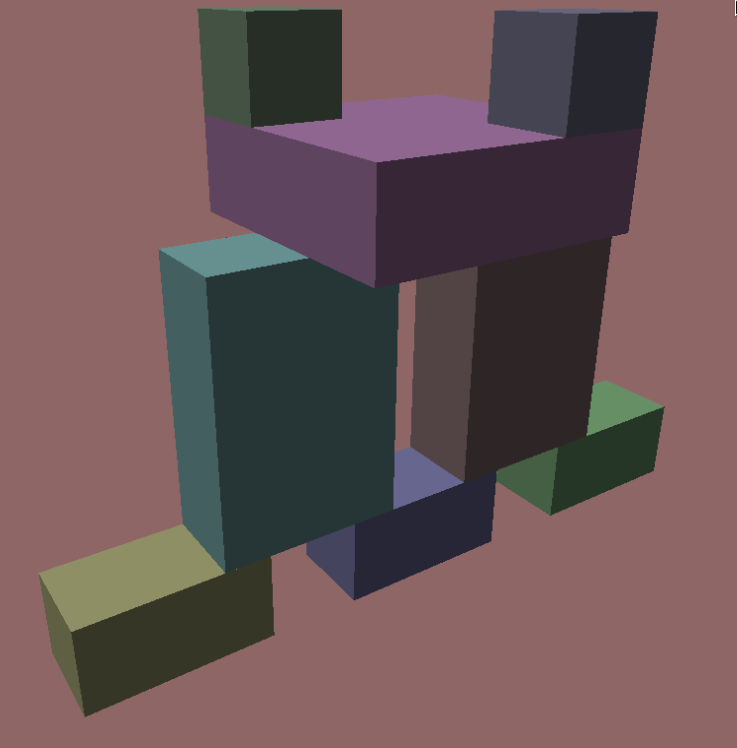
\includegraphics[width=\textwidth]{good_pic.png}
        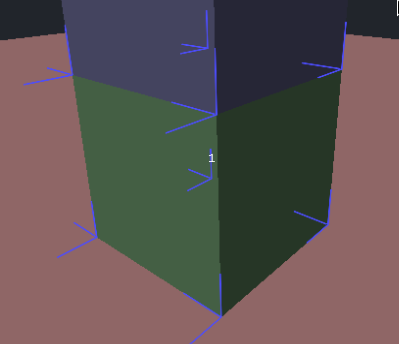
\includegraphics[width=0.3\textheight]{good_pic2.png}
    \end{column}
\end{columns}
\end{frame}

\begin{frame}
\frametitle{Как выглядит контакт?}
\begin{columns}    
    \begin{column}{0.7\textwidth}
        В точке контакта есть:
        \begin{itemize}
            \item Плосность контакта
            \item Относительное ускорение
            \item Коэффициент трения
        \end{itemize}
    \end{column}

    \begin{column}{0.3\textwidth}
        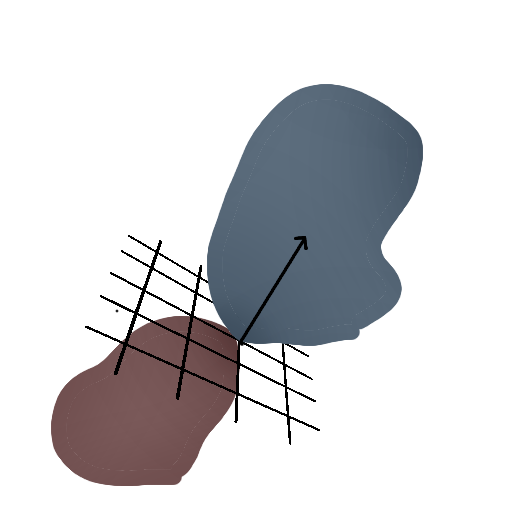
\includegraphics[height=0.3\textheight]{draw1.png}
        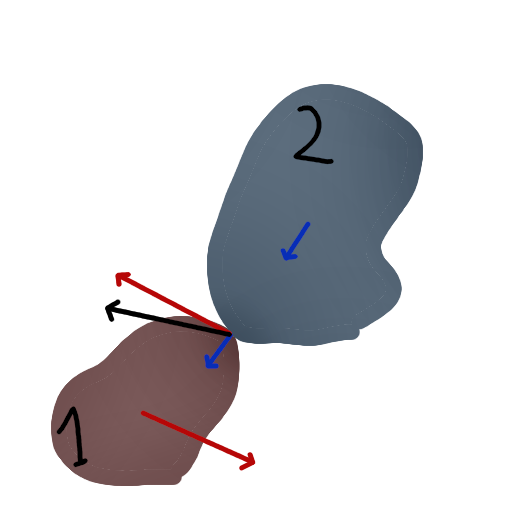
\includegraphics[height=0.3\textheight]{draw2.png}
        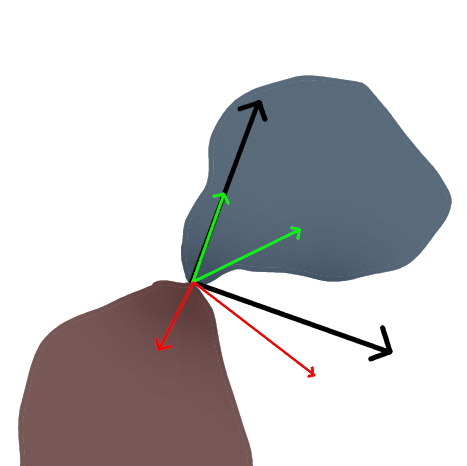
\includegraphics[height=0.25\textheight]{draw3.png}
    \end{column}
\end{columns}
\end{frame}

\begin{frame}
\frametitle{Формализация}
    \small
    \begin{columns}
        \begin{column}{0.5\textwidth}
            \[
            \begin{cases}
                1: f_n \ge 0 \\
                2: a_n \ge 0 \\
                3: f_n a_n = 0 \\ 
                4: \mu f_n \ge \norm{f_t} \\
                5: \norm{a_t} (\mu f_n - \norm{f_t}) = 0 \\
                6: \norm{a_t} \norm{f_t} = -(a_t \cdot f_t)
            \end{cases}
            \]
        \end{column}

        \begin{column}{0.5\textwidth}
            $f_n$ -- величина силы нормальной (скаляр)
            
            \medskip
            $a_n$ -- относительное ускорение в направлении нормали (скаляр)
            
            \medskip
            $f_t$ -- сила трения (2D вектор в плоскости контакта)
            
            \medskip
            $a_t$ -- относительное ускорение в плоскости контакта (тоже 2D вектор)
        \end{column}
    \end{columns}

    \begin{enumerate}
        \item Сила нормальная применяется в нужную сторону
        \item Нет проникновения одного тела в другое
        \item Если тела отдаляются, то силы применять и так уже не надо.
        \item Сила трения ограничена силой нормальной
        \item Если есть проскальзывание, то сила трения по величина максимальна.
        \item Сила трения направлена против ускорения (если оно есть)
    \end{enumerate}
\end{frame}

\begin{frame}
\small
\frametitle{Формализация. Как силы влияют на ускорение?}
    
    Хотим узнать, как влияет некоторая сила на ускорение какой-то точки тела.

    \begin{block}{Что известно}
        $c$ -- центр масс тела.
        
        $r_1$ -- точка, в которой применяется сила.
        
        $r_2$ -- интересующая нас точка.
        
        $f$ -- направление применения силы.
        
        $m, I$ -- масса тела и его тензор инерции.
    \end{block}

    \begin{block}{Вычисляем}
        $a_{lin} = f/m$ -- линейный вклад силы в ускорение.
        
        $t = (r_1 - c) \times f$ -- крутящий момент.

        $a_{ang} = I^{-1} t$ -- угловой вклад силы в ускорение.

        $a = a_{lin} + a_{ang}$
    \end{block}
\end{frame}

\begin{frame}
\frametitle{Формализация. Проецируем все силы}
    Отображение линейное!

    \[A
    \begin{pmatrix} f_1 \\ f_2 \\ \vdots \\ f_{N} \end{pmatrix}
    =
    \begin{pmatrix} a_1 \\ a_2 \\ \vdots \\ a_M \end{pmatrix}
    \]
\end{frame}

\begin{frame}[t]
\frametitle{Формализация. Как решать?}
    \small
    \[
    \begin{cases}
        f_n \ge 0 \\
        a_n \ge 0 \\
        f_n a_n = 0 \\ 
        \mu f_n \ge \norm{f_t} \\
        \norm{a_t} (\mu f_n - \norm{f_t}) = 0 \\
        \norm{a_t} \norm{f_t} = -(a_t \cdot f_t)
    \end{cases}
    \]

    \begin{itemize}
        \item Ограничения выпуклые?
        \item Ограничения линейные?
    \end{itemize}
\end{frame}


\begin{frame}[t]
\frametitle{Формализация. Как решать?}
    \small
    Перефразируем первые 3 условия:

    $0 \le a \perp b \ge 0  \iff  \{ a \ge 0, b \ge 0, ab = 0 \}$

    \[
    \begin{cases}
        0 \le f_n \perp a_n \ge 0 \\
        \mu f_n \ge \norm{f_t} \\
        \norm{a_t} (\mu f_n - \norm{f_t}) = 0 \\
        \norm{a_t} \norm{f_t} = -(a_t \cdot f_t)
    \end{cases}
    \]


\end{frame}

\begin{frame}[t]
\frametitle{Формализация. Как решать?}
    \small
    Перефразируем первые 3 условия:

    $0 \le a \perp b \ge 0  \iff  \{ a \ge 0, b \ge 0, ab = 0 \}$

    \[
    \begin{cases}
        0 \le f_n \perp a_n \ge 0 \\
        \mu f_n \ge |f_t| \\
        \norm{a_t} (\mu f_n - |f_t|) = 0 \\
        \norm{a_t} |f_t| = -(a \cdot t) \cdot f_t
    \end{cases}
    \]

    Выберем направление силы трения произвольно.
    Тогда $f_t$ превращается в скаляр. $t$ -- направление силы
\end{frame}



\begin{frame}[t]
\frametitle{Формализация. Как решать?}
    \small
    Перефразируем первые 3 условия:

    $0 \le a \perp b \ge 0  \iff  \{ a \ge 0, b \ge 0, ab = 0 \}$

    \[
    \begin{cases}
        0 \le f_n \perp a_n \ge 0 \\
        \mu f_n \ge f_{t+} + f_{t-} \\
        \norm{a_t} (\mu f_n - f_{t+} - f_{t-}) = 0 \\
        \norm{a_t} (f_{t+} + f_{t-}) = -(a \cdot t) \cdot (f_{t+} - f_{t-}) \\
        f_{t+} \perp f_{t-}
    \end{cases}
    \]

    Выберем направление силы трения произвольно.
    Тогда $f_t$ превращается в скаляр. $t$ -- направление силы

    Разобьем $f_t$ на две части: $f_{t+}$, $f_{t-}$. Первая применяется в положительном направлении. Вторая -- в отрицательном.
    Наложим на них требование $f_{t+} \perp f_{t-}$.
    Тогда $f_t = f_{t+} - f_{t-}$, $|f_t| = f_{t+} + f_{t-}$
\end{frame}


\begin{frame}[t]
\frametitle{Формализация. Как решать?}
    \small
    Перефразируем первые 3 условия:

    $0 \le a \perp b \ge 0  \iff  \{ a \ge 0, b \ge 0, ab = 0 \}$

    \[
    \begin{cases}
        0 \le f_n \perp a_n \ge 0 \\
        \mu f_n \ge f_{t+} + f_{t-} \\
        \norm{a_t} (\mu f_n - f_{t+} - f_{t-}) = 0 \\
        \norm{a_t} (f_{t+} + f_{t-}) = -(a \cdot t) \cdot (f_{t+} - f_{t-}) \\
        f_{t+} \perp f_{t-} \\
        \\
        \beta \ge 0 \\
        0 \le (a \cdot t) + \beta \perp f_{t+} \ge 0 \\ 
        0 \le -(a \cdot t) + \beta \perp f_{t-} \ge 0 
    \end{cases}
    \]

    Введём дополнительную переменную $\beta$ и добавим 2 условия. Индикаторы наличия движения.
    Условия 4 и 5 становятся бесполезными.

\end{frame}



\begin{frame}[t]
\frametitle{Формализация. Как решать?}
    \small
    Перефразируем первые 3 условия:

    $0 \le a \perp b \ge 0  \iff  \{ a \ge 0, b \ge 0, ab = 0 \}$

    \[
    \begin{cases}
        0 \le f_n \perp a_n \ge 0 \\
        \mu f_n \ge f_{t+} + f_{t-} \\
        \norm{a_t} (\mu f_n - f_{t+} - f_{t-}) = 0 \\
        \\
        \beta \ge 0 \\
        0 \le (a \cdot t) + \beta \perp f_{t+} \ge 0 \\ 
        0 \le -(a \cdot t) + \beta \perp f_{t-} \ge 0 
    \end{cases}
    \]

    Условие 3 гласит: если скольжение есть, то сила трения по величине максимальна.
    Это условие можно переписать через $\beta$
\end{frame}


\begin{frame}[t]
\frametitle{Формализация. Как решать?}
    \small
    Перефразируем первые 3 условия:

    $0 \le a \perp b \ge 0  \iff  \{ a \ge 0, b \ge 0, ab = 0 \}$

    \[
    \begin{cases}
        0 \le f_n \perp a_n \ge 0 \\
        \mu f_n \ge f_{t+} + f_{t-} \\
        0 \le \mu f_n - f_{t+} - f_{t-} \perp \beta \ge 0 \\
        \\
        0 \le (a \cdot t) + \beta \perp f_{t+} \ge 0 \\ 
        0 \le -(a \cdot t) + \beta \perp f_{t-} \ge 0 
    \end{cases}
    \]

    Условие 2 теперь, кстати, тоже бесполезное.
\end{frame}



\begin{frame}[t]
\frametitle{Формализация. Как решать?}
    \small
    Перефразируем первые 3 условия:

    $0 \le a \perp b \ge 0  \iff  \{ a \ge 0, b \ge 0, ab = 0 \}$

    \[
    \begin{cases}
        0 \le f_n \perp a_n \ge 0 \\
        0 \le \mu f_n - f_{t+} - f_{t-} \perp \beta \ge 0 \\
        0 \le (a \cdot t) + \beta \perp f_{t+} \ge 0 \\ 
        0 \le -(a \cdot t) + \beta \perp f_{t-} \ge 0 
    \end{cases}
    \]

    Теперь все ограничения, кроме условий дополняющей нежесткости, линейны.
    С этой задачей смогут справиться солверы LCP (Linear Complementarity problem).
    \medskip
    
    Перебирать направления сил трения и выбирать лучшее решение?
\end{frame}

\begin{frame}
    \small
    \frametitle{Выбор лучшего решения}

    Для каждого решения, для каждого контакта имеем $a$ -- относительное ускорение (3D вектор).
    
    Рассматриваем его в базисе контакта:  $a_n$ (скаляр), $a_t$ (2D вектор).

    Штрафуем за несоблюдение оригинальных условий:

    \[
    \begin{matrix}
        f_n \ge 0 - \text{OK!} && \\
        a_n \ge 0 - \text{OK!} &&\\
        f_n a_n = 0 - \text{OK!} && \\ 
        \mu f_n \ge \norm{f_t} - \text{OK!} && \\
        \norm{a_t} (\mu f_n - \norm{f_t}) = 0 - \textbf{NOT OK!} && |\norm{a_t} (\mu f_n - \norm{f_t})| \\
        \norm{a_t} \norm{f_t} = -(a_t \cdot f_t) - \textbf{NOT OK!} && |\norm{a_t} \norm{f_t} + (a_t \cdot f_t)|
    \end{matrix}
    \]
\end{frame}

\begin{frame}
    \frametitle{Результаты}
    2 кирпича. Без ветра.
    \begin{columns}
        \begin{column}{0.7\textwidth}
            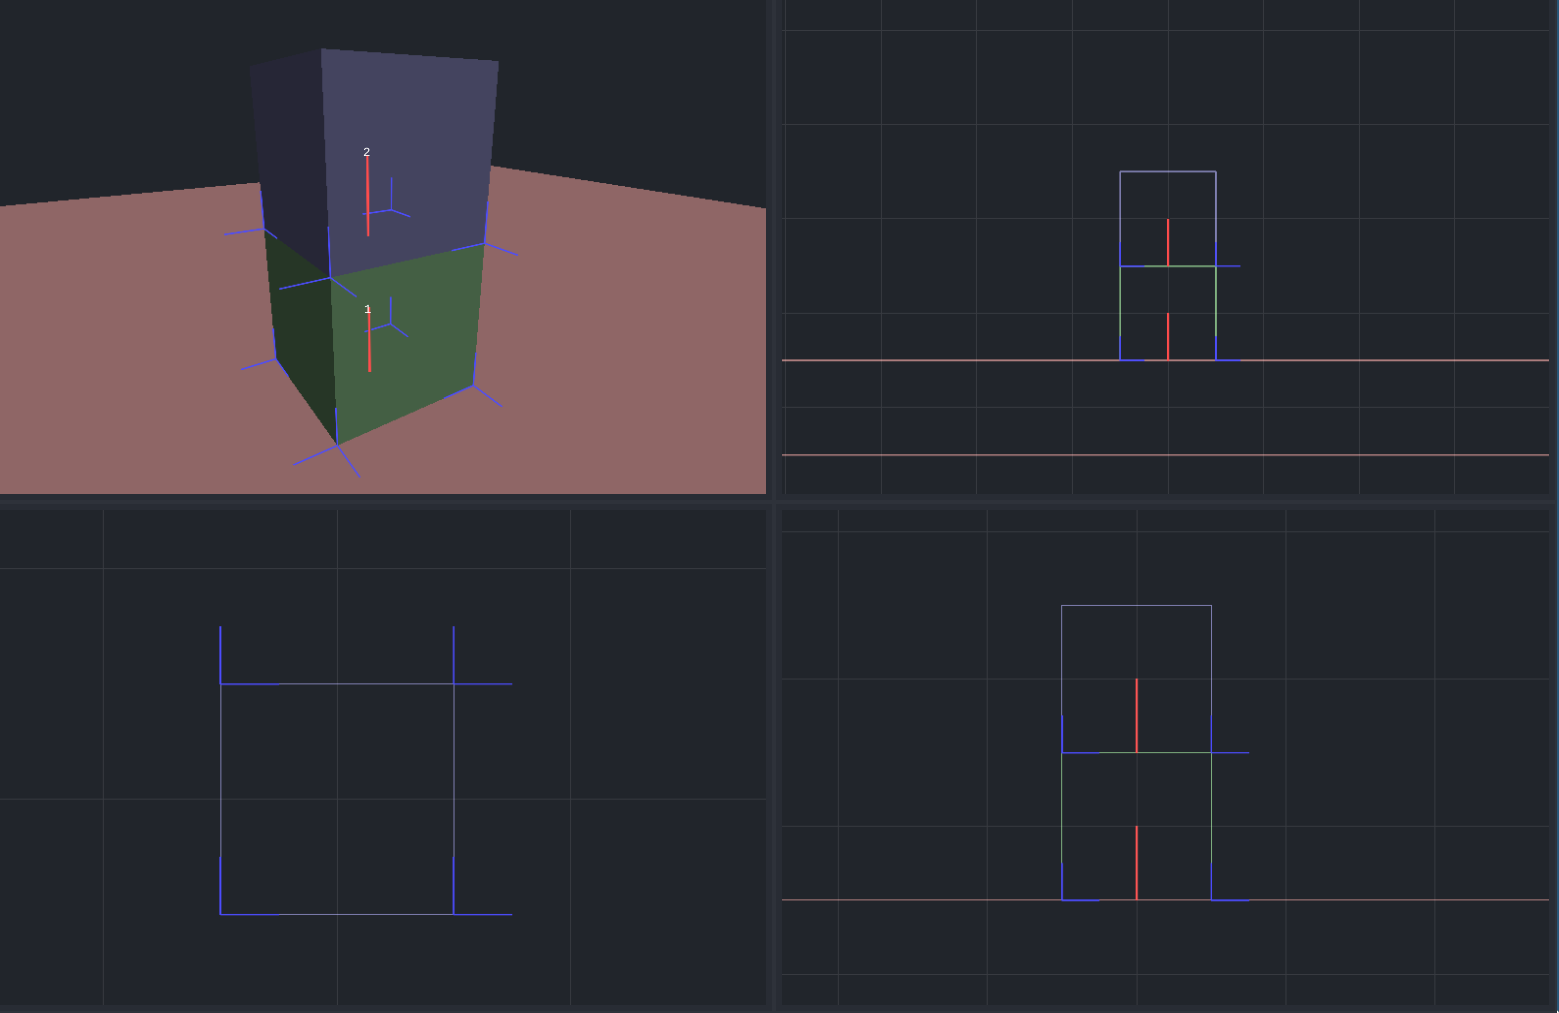
\includegraphics[width=\textwidth]{result_i2.png}
        \end{column}
        \begin{column}{0.3\textwidth}
            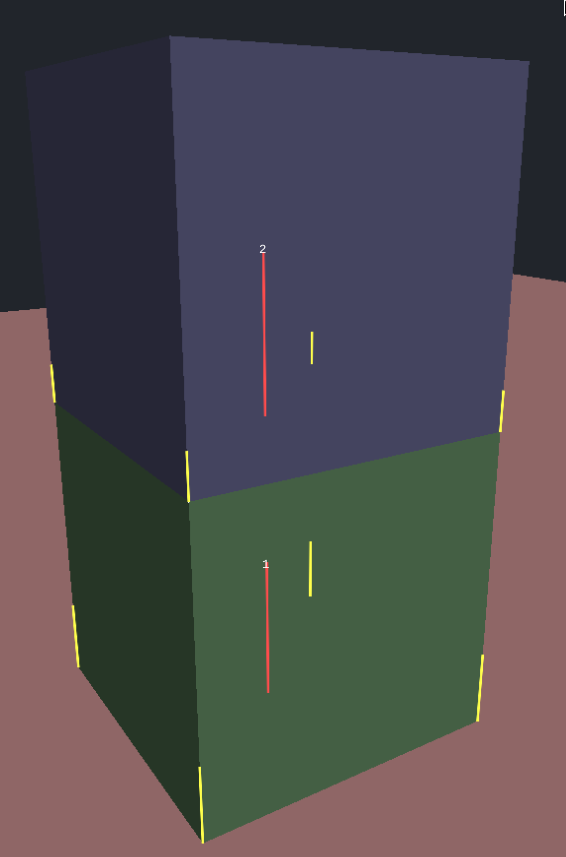
\includegraphics[width=\textwidth]{result_o2.png}
        \end{column}
    \end{columns}
\end{frame}


\begin{frame}
    \frametitle{Результаты}
    2 кирпича. Боковой ветер.
    \begin{columns}
        \begin{column}{0.7\textwidth}
            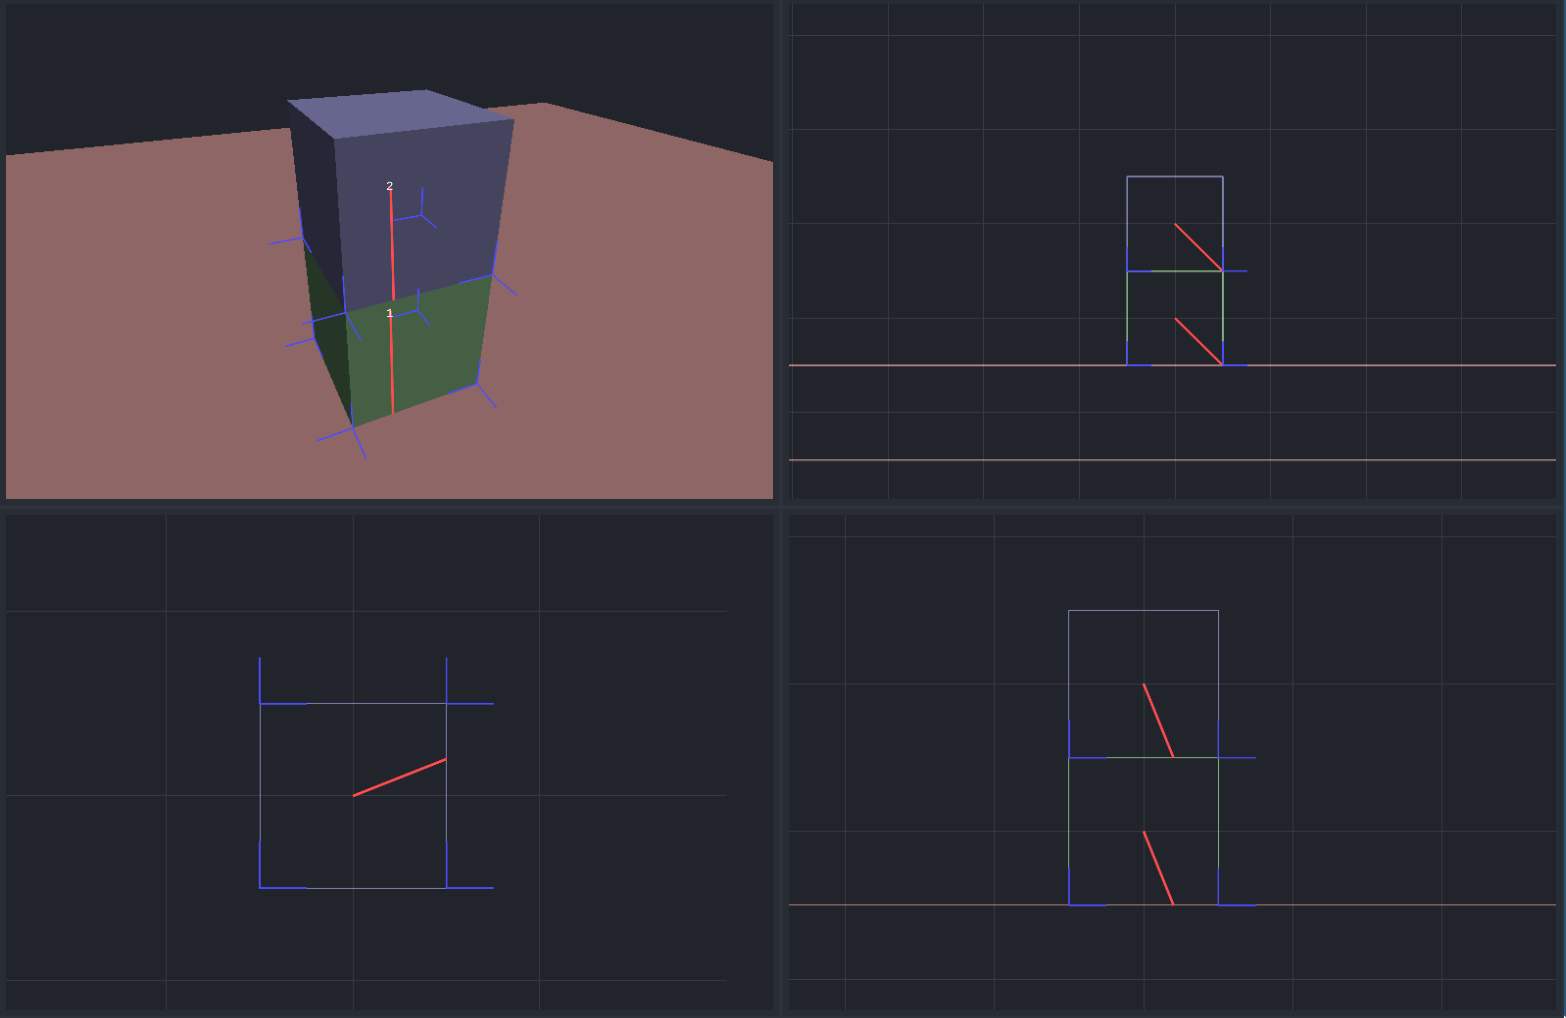
\includegraphics[width=\textwidth]{result_i1.png}
        \end{column}
        \begin{column}{0.3\textwidth}
            
\includegraphics[width=\textwidth]{result_o1.png}
        \end{column}
    \end{columns}
\end{frame}



\begin{frame}
    \frametitle{Результаты}
    Кирпич свисает.
    \begin{columns}
        \begin{column}{0.5\textwidth}
            
\includegraphics[width=\textwidth]{result_i3_1.png}
            
\includegraphics[width=\textwidth]{result_i3_2.png}
        \end{column}
        \begin{column}{0.5\textwidth}
            
\includegraphics[width=\textwidth]{result_i3_3.png}
        \end{column}
    \end{columns}
\end{frame}


\begin{frame}
    \frametitle{Результаты}
    У передних точек коэфф. трения меньше, чем у задних. Ветер.
    
\includegraphics[width=\textwidth]{result_i4.png}
\end{frame}

\begin{frame}
    \frametitle{Результаты}
    Масса верхнего кипчича 1 vs 20.

    \begin{columns}
        \begin{column}{0.5\textwidth}
            
\includegraphics[width=\textwidth]{result_i5_2.png}
        \end{column}
        \begin{column}{0.5\textwidth}
            
\includegraphics[width=\textwidth]{result_i5_1.png}
        \end{column}
    \end{columns}
\end{frame}


\begin{frame}
    \centering
    Конец
\end{frame}


\end{document}